% Figure 2.3 (Session 2): the conserved S^z_tot of the Heisenberg chain of L = 6: the blocks, the
% Zeeman fan of the lowest level of each sector, and the magnetization staircase.
% The image is rendered by figures/blender/s2_3_sz_blocks.py; the coordinates of the labels
% come from figures/blender/out/sz_blocks_anchors.tex. Compile with:
%   pdflatex sz_blocks.tex ; result moves to ../quantum_magnetism/sz_blocks.pdf
\documentclass[11pt,tikz,border=0pt]{standalone}
\usepackage{amsmath,amssymb,graphicx,braket}
\usepackage{xcolor}
\definecolor{coursedark}{HTML}{1B2A4A}
\definecolor{costamber}{HTML}{B8620A}
\newlength{\figw}\setlength{\figw}{16.19cm}   % the text width of the notes (letter, 2.7 cm margins), so labels print at size

\begin{document}
\begin{tikzpicture}[lbl/.style={font=\small, text=coursedark}, dim/.style={font=\footnotesize, text=coursedark}]
  \node[anchor=south west, inner sep=0pt] at (0,0)
    {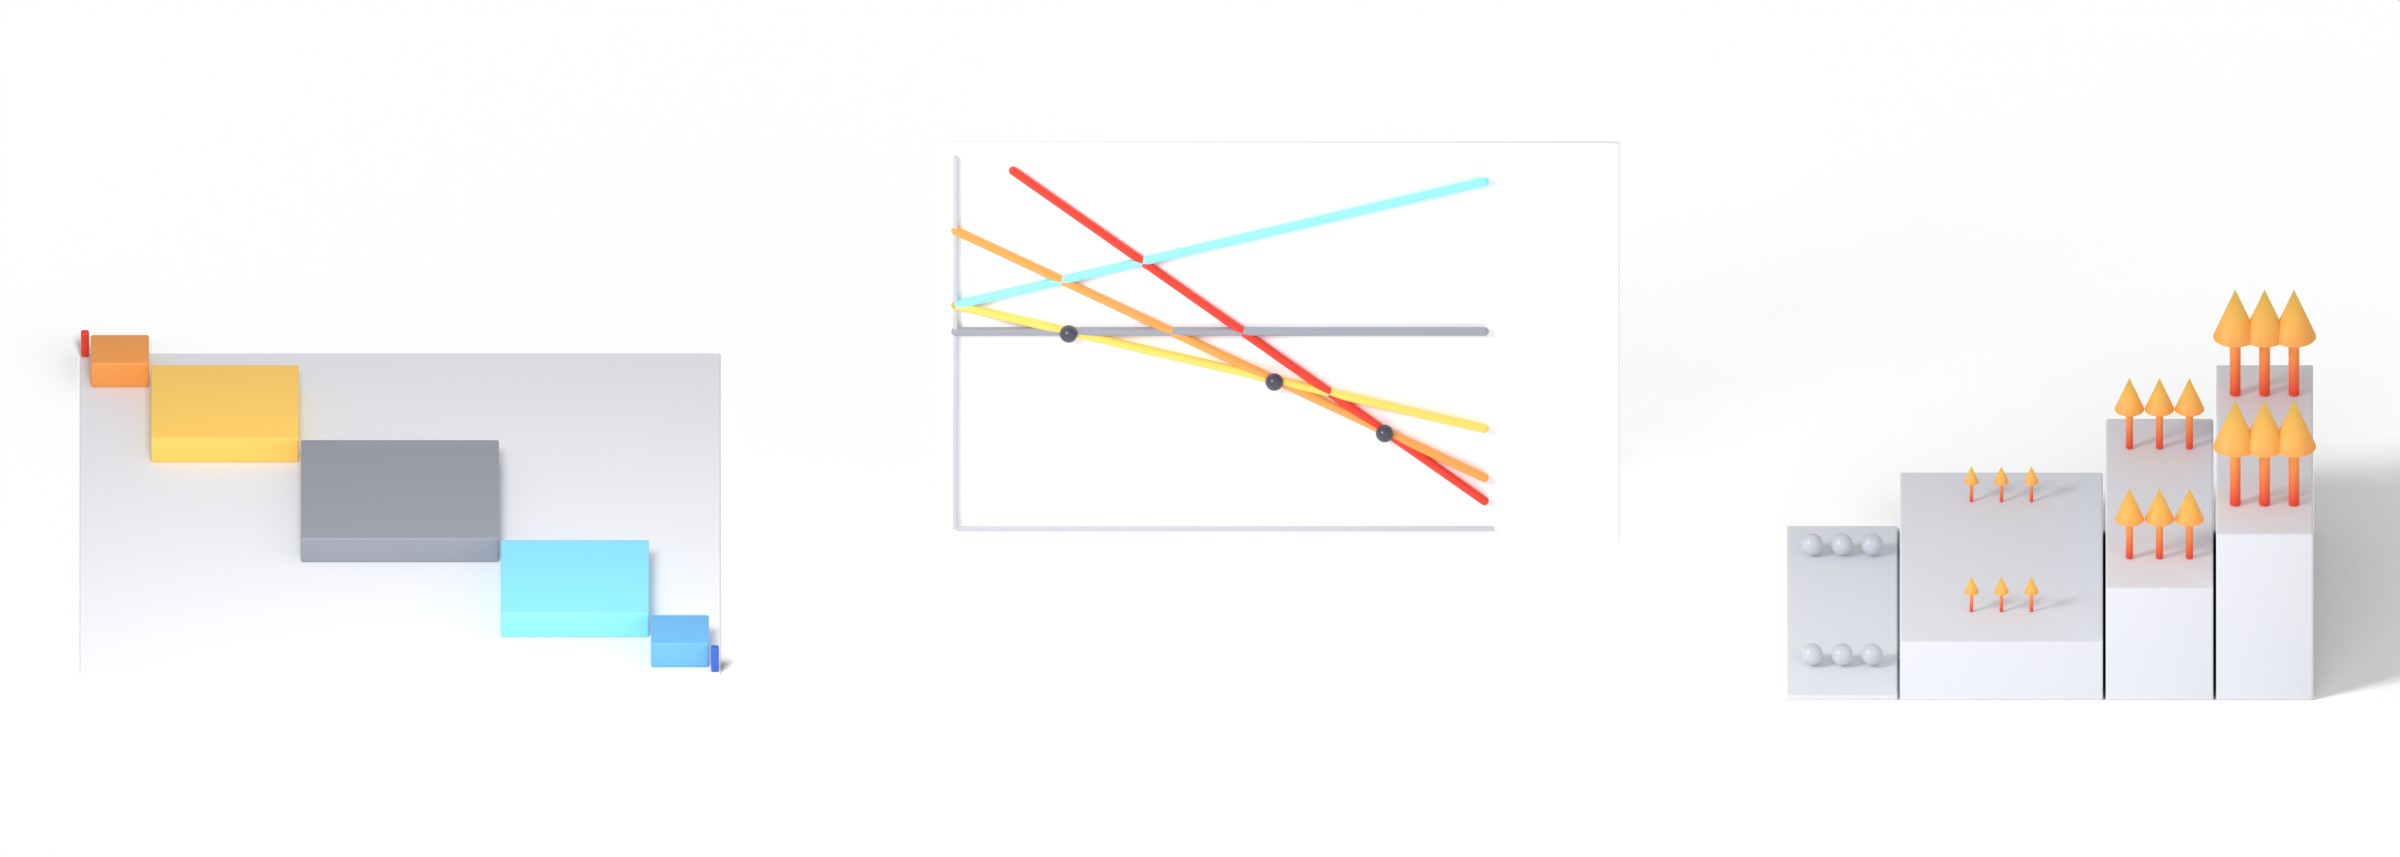
\includegraphics[width=\figw]{../blender/out/sz_blocks.jpg}};
  %% written by figlib.py; x and y in units of the image width
\coordinate (dim3) at (0.0308\figw,0.2089\figw);
\coordinate (dim2) at (0.0350\figw,0.1964\figw);
\coordinate (dim1) at (0.0600\figw,0.1652\figw);
\coordinate (dim0) at (0.1225\figw,0.1235\figw);
\coordinate (dim-1) at (0.2058\figw,0.0922\figw);
\coordinate (dim-2) at (0.2683\figw,0.0797\figw);
\coordinate (dim-3) at (0.2933\figw,0.0777\figw);
\coordinate (a) at (0.0333\figw,0.2774\figw);
\coordinate (labA) at (0.1667\figw,0.0505\figw);
\coordinate (m-1) at (0.6185\figw,0.2814\figw);
\coordinate (m0) at (0.6185\figw,0.2190\figw);
\coordinate (m1) at (0.6185\figw,0.1785\figw);
\coordinate (m2) at (0.6185\figw,0.1581\figw);
\coordinate (m3) at (0.6185\figw,0.1484\figw);
\coordinate (b) at (0.3167\figw,0.2957\figw);
\coordinate (Eb) at (0.3981\figw,0.2918\figw);
\coordinate (Bb) at (0.6227\figw,0.1369\figw);
\coordinate (labB) at (0.5083\figw,0.0505\figw);
\coordinate (pl0) at (0.7675\figw,0.0658\figw);
\coordinate (pl1) at (0.8339\figw,0.0882\figw);
\coordinate (pl2) at (0.8998\figw,0.1106\figw);
\coordinate (pl3) at (0.9436\figw,0.1330\figw);
\coordinate (c) at (0.7333\figw,0.2957\figw);
\coordinate (labC) at (0.8542\figw,0.0505\figw);

  \node[lbl, font=\normalsize, anchor=west] at (a) {(a)};
  \node[lbl, font=\normalsize, anchor=west] at (b) {(b)};
  \node[lbl, font=\normalsize, anchor=west] at (c) {(c)};
  \foreach \m/\d in {3/1, 2/6, 1/15, 0/20, -1/15, -2/6, -3/1}
    \node[dim, anchor=north east, inner sep=1pt] at (dim\m) {$\d$};
  \node[lbl, anchor=north, align=center] at (labA) {$2^6\times2^6$ matrix, one block per $m$};
  \node[lbl, anchor=north, align=center] at (labB) {lowest level of each $m$ against $B$};
  \foreach \m in {0,1,2,3} \node[dim, anchor=north] at (pl\m) {$m=\m$};
  \node[lbl, anchor=north, align=center] at (labC) {ground-state $m$ against $B$};
  \node[lbl, anchor=west] at (m0) {$m=0$};
  \node[lbl, anchor=north west, inner sep=1pt] at (m3) {$m=3$};
  \node[lbl, anchor=west] at (m-1) {$m=-1$};
  \node[lbl, anchor=west] at (m1) {$m=1$};
  \node[lbl, anchor=west] at (m2) {$m=2$};
  \node[lbl, anchor=south] at (Eb) {$E$};
  \node[lbl, anchor=north] at (Bb) {$B$};
\end{tikzpicture}
\end{document}
